\pdfoutput=1
% arXiv requires \pdfoutput=1 inside the first five lines to select pdfTeX.
% IEEEtran V1.8b (2015/08/26). Bundle IEEEtran.cls and main.bbl in the arXiv
% tarball: arXiv runs neither bibtex nor biber on an uploaded .bib file.
%
% No em dash or en dash appears in this document. In LaTeX source that means
% the triple-hyphen and double-hyphen ligatures are never used, including in
% bibliography page ranges, where a single hyphen is used instead.
\documentclass[conference]{IEEEtran}

\usepackage{etoolbox}
% IEEEtran.cls hardcodes a triple-hyphen ligature after "Abstract" and after
% "Index Terms", and IEEEtran.bst emits one for a repeated author and turns
% page ranges into the double-hyphen ligature. This project forbids both
% rendered dashes outright. The class file itself is NOT edited, because a
% modified IEEEtran.cls would be a format non-conformance a reviewer or an
% automated check would be right to flag. Instead the two class macros are
% patched in this preamble to use a colon, and the bibliography is
% post-processed by build.sh after bibtex runs. If either patch stops
% matching a future IEEEtran, the \PackageError below stops the build rather
% than letting a dash through silently.
\makeatletter
\patchcmd{\abstract}{---}{:\ }{}{\PackageError{titan}{abstract dash patch failed}{}}% dash-check-allow-this-line-removes-a-dash
\patchcmd{\IEEEkeywords}{---}{:\ }{}{\PackageError{titan}{keywords dash patch failed}{}}% dash-check-allow-this-line-removes-a-dash
\makeatother

\usepackage{graphicx}
\graphicspath{{../figures/}}
\usepackage{booktabs}
\usepackage{amsmath}
\usepackage{url}
\usepackage[hidelinks]{hyperref}

\begin{document}

\title{When a Full Barrier Beats a Store-Release, and When It Does Not:\\
A Pre-Registered Measurement Study on a Fanless Apple M4,\\
and Eight Pre-Registered Thresholds That Did Not Test Their Claims}

\author{\IEEEauthorblockN{Anonymous Author(s)}
\IEEEauthorblockA{Submission under double-blind review}}

\maketitle
\bstctlcite{bstctl:titan}

\begin{abstract}
In a single-producer single-consumer ring the memory-ordering operation is a
large fraction of the loop, not a rounding error on it. On a fanless
Apple M4 that fraction is 95.3 percent, measured against an unordered cost
floor that is not a correct ring.
Replacing a store-release with a \texttt{dmb ish} barrier and a plain store
costs 2.5766 times fewer cycles per message when the cursor line is contended
and 2.7008 times more once it is resident in L1, each in 30 of 30 independent
launches. That a store-release can cost more than a stronger barrier has been
reported before without a condition; we measure three that decide it. Crossing the halves of the acquire-release pair localises the effect
entirely to the store side, and ring capacity reverses it again,
non-monotonically. Most of the difference is time spent waiting after an L1D
miss, a waiting ratio of 0.2338, whose cause we do not identify: controlling
for duration leaves a coherence component too small to explain it. Separately,
arrival clustering moves the tail further than any ordering construct here, and
the Fano factor of counts predicts a ratio of 1.040 where the squared
coefficient of variation of interarrival times predicts 7.444 and the measured
ratio reaches 13.5030.

All of it comes from a pre-registered protocol, 94 hypothesis rows and five
exploratory calibrations, with thresholds fixed before each run and an exact
sign test over launches. That protocol also failed, and how it failed is the
second contribution. Eight of those thresholds were precise, checkable,
honoured exactly as written, and not tests of the claims they were written for.
Pre-registration fixes a threshold; it does not aim one. We name the failure
mode, give the eight instances, and publish the defect register and eleven
automated checks that refuse a manuscript whose numbers or figures disagree
with the files they come from.
\end{abstract}

\begin{IEEEkeywords}
memory consistency, Apple silicon, AArch64, lock-free queues, performance
measurement, measurement bias, hardware performance counters,
pre-registration, reproducibility, artifact evaluation
\end{IEEEkeywords}

\section{Introduction}

A feed handler reconstructing a limit order book from an exchange multicast
feed~\cite{maciejewski2026cme} spends its time in a loop of a few
instructions: read the producer's cursor, read a slot, update book state,
publish the consumer's cursor. The cursors are shared between two cores, so
each read and each publish carries a memory-ordering obligation discharged by
an instruction the programmer selects through a source-level annotation. The
cost of that obligation matters because of what a few hundred nanoseconds buys.
Budish et al.~\cite{budish2015hft} argue the speed race is built into
continuous-time market design, and Aquilina et
al.~\cite{aquilina2022quantifying} measure races directly from exchange message
data, finding roughly one race per minute per symbol in FTSE 100 stocks with
the modal race decided in 5 to 10 microseconds. A fixed cost of a few hundred
nanoseconds in a cross-core hand-off is a visible fraction of that, spent
before any strategy logic runs, and the same arithmetic holds with no exchange
in it, since Dean and Barroso~\cite{dean2013tail} show a small per-stage
component dominates once enough stages compose.

The prevailing guidance for such a loop is that the weak orderings are cheap
and should be preferred to sequential consistency, and that an explicit full
barrier is the expensive option of last resort. That guidance is sound as a
summary of the architecture manuals. It is also, on the machine measured here,
wrong about which of two correct rings is faster, wrong by a factor of 2.57,
and wrong in the opposite direction depending on whether a single cache line
happens to be resident.

The nearest prior work makes the gap explicit. Khayet and
Morrison~\cite{khayet2026arm} measure Apple M1 and M4 under Apple's
runtime-configurable total store order mode against native Arm mode across 49
application workloads, and conclude that the Arm memory model carries no
inherent performance advantage on Apple silicon, with typical execution times
within about 3 percent. They state that they leave the performance of atomic
read-modify-write operations and memory barriers to future work, on the stated
assumption that modern concurrent software is not bottlenecked on
synchronization. For the workloads they measure, that assumption is reasonable.
For the loop measured here it is false, and we measure the fraction rather than
asserting it: with ordering removed entirely the loop runs at 10.185 cycles per
message against 218.880 with an acquire-release pair, so 95.3 percent of the
contended loop is ordering. The unordered arm is a cost floor and not a correct
ring, and we report it as such: it failed its checksum in every one of its 180
epochs while each correct ring passed in 180 of 180. The fraction therefore
bounds what ordering costs, and does not name a cheaper ring that exists.

\subsection{Contributions}

\begin{itemize}
\item \textbf{The condition that governs the store-release anomaly.} That a
store-release can cost more than a stronger barrier is already
reported~\cite{liu2020barriers,arden2023riscv}, without stating when, and
Liu et al. recommend measuring it for that reason. The first condition measured
here is caching state, and a second, ring capacity, appears in
Section~\ref{sec:cycles} and reverses the comparison again: substituting \texttt{dmb ish} and a plain store for the release
store costs 2.5766 times fewer cycles per message when the cursor line is
contended and 2.7008 times more when it is resident in L1, each at 30 of 30
launches, so the comparison changes sign rather than magnitude. Two runs with
different epoch counts agree on the contended figure to one part in a thousand.
The obvious explanation is excluded by the counters, within the scope the
counters actually cover: on the consuming thread, the barrier arm carries more
L1D load misses than the acquire-release arm in every configuration and is
faster when contended anyway. Counting is per thread on this unit and the
measuring thread ran the consumer, so this bounds the consumer's load traffic
and says nothing about the producer's.

\item \textbf{The effect is localised to the store side, by a pre-registered
cross of the two halves.} We measure four correct rings formed by crossing the
load side and the store side independently, so that each arm still carries
acquire semantics on every cursor read and release semantics on every publish,
whether from the instruction or from an adjacent barrier. The store-side share
of the total difference, taken as the median of the per-launch ratios rather
than as the ratio of the medians, which is 1.0728, is 1.0702 with a bootstrap
interval of [1.0621, 1.0866], at or above the pre-registered 0.70 in 30 of 30 launches; the
load-side share is 0.2797 and reaches that threshold in 0 of 30. The two
substitutions are strongly sub-additive, and adding the load-side barrier on
top of the store-side barrier costs 9.067 cycles.

\item \textbf{The ranking of all four correct rings reverses between caching
configurations.} Contended, the order is 85.269, 94.336, 183.800 and 218.880
cycles per message; L1-resident, it is 8.021, 8.053, 20.567 and 22.120. The
cheapest contended ring is the dearest resident one.

\item \textbf{A measurement hazard specific to heterogeneous consumer silicon.}
The core clock on this part tracks elapsed busy time rather than work
completed. A comparison that is stable in principle therefore moves by a stated
16.33 times between 200,000 and 10,000,000 messages, and the ordering that is
cheapest at the short run length is the dearest at the long one. This is a post-2009 instance of the
phenomenon named by Mytkowicz et al.~\cite{mytkowicz2009wrong}, from a bias
source that did not exist on a general-purpose CPU at that time.

\item \textbf{The lead results reproduce across time and a platform revision,
not merely across a re-analysis.} The barrier cross was re-run in full, 30
fresh launches three days after the original, on a macOS build the original
did not run on. The contended inversion returned at 2.5401 against a published
2.57, the resident one at 2.5146 against 2.75 with its sign intact, and both
caching rankings came back identical arm for arm. The replication was
registered with its tolerances before it ran and retains every record, so each
statistic above is recomputable from committed data rather than quoted from a
summary.

\item \textbf{A protocol built so the conclusions survive the hazard.} Every
comparison here is pre-registered with pass and fail thresholds fixed before
the run, measured over independent process launches, 30 for every comparison
but the run-length sweep, which used 20 at each of its four message counts,
paired within each launch and tested with an exact two-sided sign test for
which 21 of 30 is the p < 0.05 threshold. Every figure regenerates from the committed
measurement files with one command.
\end{itemize}

\subsection{What this paper does not claim}

A third run settles which numbers to trust. The replication was measured in
nanoseconds, because the counters require root and an unattended script must
not carry a password prompt, and a nanosecond ratio is a work ratio only if the
arms ran at similar clocks. Reading the counters directly over 30 launches and
900 records gives 2.5766 contended and 2.7008 resident, each at 30 of 30.
The frequency difference between the compared arms is 1.0086 contended and
1.0611 resident, which accounts for the gap between the two readings. The
registered check on frequency spread was written over all five arms rather than
the compared pair and failed at 1.1922, driven by the unordered cost floor.
That specification fault is recorded rather than repaired after the fact, and
the consequence registered before the run stands: the figures above are
cycles.
Across the committed runs the measured clock spans a factor of four, and every
table carries the clock measured in its own arm rather than a nominal figure,
so the cycle comparisons are not frequency differences in disguise.

The mechanism behind the store-side result is a hypothesis and reported as one.
A release store must not become visible before prior accesses are observable,
and with a coherence miss in flight the measured cost is consistent with the
store stalling until that miss completes, where a barrier followed by a plain
store pays a fixed cost once and retires into the store buffer. That would
explain both the saving when the line is contended and the penalty when it is
not. It is not established, and a queue-occupancy explanation is not excluded:
a barrier changes how far the producer runs ahead, and instrumenting occupancy
inside the hot loop would perturb the quantity measured.

The results are from one Apple M4 in one fanless chassis, one ring, one padding
and one wait strategy, on performance cores. A cross-architecture control on
x86-64 is reported with the limitation that the host is virtualized and exposes
no frequency-scaling interface, so there the absence of the run-length effect
and the invisibility of the clock cannot be told apart.

\section{Related Work}

\textbf{What the models specify, and what they omit.} The ARMv8 concurrency
model has a formal semantics. Alglave et al.~\cite{alglave2014herding} give an
axiomatic framework covering ARM, Power and x86; Pulte et
al.~\cite{pulte2018simplifying} document the revision to multicopy atomicity;
Batty et al.~\cite{batty2011mathematizing} do the corresponding work at the
language level the Rust annotations here inherit; and Alglave et
al.~\cite{alglave2018frightening} carry the machinery into the Linux kernel.
Together they answer whether an execution is permitted. None answers what an
ordering choice costs on a particular part, and the two questions come apart
here: the acquire-release and fenced-store arms are both permitted, both
correct, and differ in cost by a factor that changes sign with cursor
residency. Cost is not in the models' vocabulary. This paper measures that
quantity on hardware, with the semantics held fixed by the models rather than
argued about.

\textbf{Queues, bias and reporting.} The ring measured here descends from work
on cache-conscious single-producer hand-off. Giacomoni et
al.~\cite{giacomoni2008fastforward} showed the dominant cost is the cache
traffic the index variables generate, which is why the cursors here sit on
separate lines and why the capacity sweep separates slot count from footprint.
Mytkowicz et al.~\cite{mytkowicz2009wrong} established that measurement bias in
systems evaluation can reverse a conclusion and is commonplace, surveying 133
papers without finding one that adequately considered it; Curtsinger and
Berger~\cite{curtsinger2013stabilizer} randomise layout to remove it, and
Zaparanuks et al.~\cite{zaparanuks2009accuracy} show the counters themselves
carry error. Georges et al.~\cite{georges2007statistically} set the
reporting standard this paper follows, and Collberg and Proebsting~\cite{collberg2016repeatability} measured
how rarely published systems work can be rebuilt at all. The second result here
is an instance of Mytkowicz's phenomenon rather than a rediscovery of it, and
the distinction is the bias source: core frequency on this part is a function
of how long the core has been busy, not of how much work it was given, so two
implementations handed identical message counts are measured at different
clocks. Neither that source nor heterogeneous core residency existed on a
general-purpose CPU in 2009.

\textbf{The two gaps this paper fills.} Khayet and
Morrison~\cite{khayet2026arm} measure Apple silicon's runtime-configurable TSO
against native ARM mode on the M1 and M4, and explicitly leave the effect on
atomic read-modify-write and memory barrier operations to future work, on the
stated ground that modern concurrent software is generally not bottlenecked on
synchronisation. Wrenger et al.~\cite{wrenger2023tosting, wrenger2024m1}
characterise the same mode from the operating system's side. On the
single-producer single-consumer hand-off measured here the ordering operation
is 95.3 percent of the loop, which is a case where that ground does not hold,
and the question their Section~4 set aside is the one measured here on the same
silicon. Separately, the pre-registration literature in empirical science
requires both a prediction and an analysis plan~\cite{nosek2018preregistration},
and the disagreement that followed~\cite{ledgerwood2018distinguish,
nosek2018reply} concerns how binding the plan should be. Neither side reaches
the case where both halves are well formed and the plan still cannot answer the
prediction, because in those designs the mapping is usually obvious. In
measurement it is not, and eight registered thresholds in this study failed in
exactly that way. Cockburn et al.~\cite{cockburn2020threats} survey how threats
to validity are reported in computing, and queueing theory supplies the
arrival-process background~\cite{kingman1961heavy, kingman1962queues,
hawkes1971spectra, ogata1981thinning} for the schedules used in
Section~\ref{sec:cycles}.

\section{Method}
\label{sec:method}

\subsection{Platform}

Every measurement reported as ours was taken on one machine, an Apple MacBook
Air identifying as Mac16,13 with an M4 and ten cores, four of them performance
cores, under macOS 27.2.1. Two operating system builds appear in the record,
26B123 and 26B131, because the system updated between two runs partway through
the work. The consequence was measured rather than assumed: the affected result
was replicated in full on the newer build, and every registered part of it
reproduced. The toolchain is a single \texttt{rustc} 1.92.0. The part is
fanless, which is not incidental: it is the reason run length changes a
comparison here and the reason the thermal state of a run is recorded with it.

Where a second platform appears it is labelled as such and used only as a
control. Those runs are on virtualised x86-64 hosts, for which no power state
exists; their results files say so in the field rather than leaving it blank.

\subsection{The ring under measurement}

The object of study is a single-producer single-consumer ring of 1024 slots
with the cursors on separate 128-byte lines, the coherence granule on this part
rather than the 64 bytes an x86 port would use. The loop body is a cursor load,
a slot access, a cursor store and a branch, and nothing else. That smallness is
the point: it makes the ordering operation a large fraction of the work rather
than a rounding error, and it is why the premise under which Khayet and
Morrison defer barriers to future work does not hold here.

Five orderings are compared: an acquire load paired with a release store, the
same with \texttt{dmb ish} substituted on the load side alone, the store side
alone, and both, and an unordered arm. The instructions LLVM emits are recorded
by an instruction census over the compiled library rather than assumed. The
acquire-release arm compiles to \texttt{ldapur} with \texttt{stlr} on the
producer path and \texttt{ldapr} with \texttt{stlur} on the consumer path, so
both RCpc forms appear and neither path uses \texttt{ldar}. Substituting the
store side replaces the release store with \texttt{dmb ish} and a plain
\texttt{str} on both paths, adding exactly one barrier and one store to each
census; naming a single instruction for the store side would have been wrong,
because the two paths do not use the same one. The unordered arm is a cost
floor and not a candidate: it fails its checksum in 0 of 180 epochs while each
correct ring passes 180 of 180.

Each ordering runs in two caching states, cursor line contended between cores
and resident in L1, under three waiting strategies: a bare spin, a spin with
\texttt{isb}, and \texttt{wfe} on a watched address. Memory is pinned before
timing, with 4096 of 4096 pages of a 64\,MiB region resident under
\texttt{mlock} and zero faults during the hot loop, on a part whose pages are
16384 bytes. The hot loop allocates nothing, measured under a counting global
allocator rather than asserted.

\subsection{What this machine can and cannot resolve in time}

The timing facility advertises one resolution and delivers another.
\texttt{CNTFRQ\_EL0} reports 1000000000, so code trusting it computes a one
nanosecond tick, while \texttt{hw.tbfrequency} reports 24000000 and the Mach
timebase is 125/3, or 41.667 nanoseconds. We settled it by measurement: over
ten million consecutive reads of the virtual counter, 0.7558 of reads do not
advance at all and the advancing steps are multiples of roughly 41.667
nanoseconds. No claim here rests on a latency difference near that grain, and
the cycle counts carrying the central results come from the performance
monitoring unit rather than the timer.

\subsection{Hardware counters, and the boundary we measured rather than assumed}

Cycle figures come from the Apple performance monitoring unit through the
\texttt{kperf} and \texttt{kperfdata} private frameworks, loaded by
\texttt{dlopen} because they do not exist as files. The event database carries
104 events and all four used here resolve against it:
\texttt{FIXED\_CYCLES}, \texttt{FIXED\_INSTRUCTIONS},
\texttt{L1D\_CACHE\_MISS\_LD} and \texttt{BRANCH\_MISPRED\_NONSPEC}. Reads are
bracketed by \texttt{dmb ish} and \texttt{isb sy} so work inside the measured
region cannot retire outside it.

Counter values are not taken on trust. Weaver and
McKee~\cite{weaver2008trusted} showed that even retired-instruction counters
vary run to run, and three counters this study attempted to use measure nothing
in this workload. Counting is per thread and the counters belong to whichever
thread reads them; here that thread ran the consumer, so every counter figure
describes the consuming side. We state this because we did not state it soon
enough: a registered threshold on retired store misses was written against the
consumer while the arms differ in the producer's store, and returned zero on
every arm of nine hundred records. A diagnostic driving three passes of known
L1D behaviour confirms the event counts correctly, so the zero was a correct
measurement of the wrong quantity. That threshold is recorded as unevaluable
rather than passed.

Three properties of the apparatus were measured. \emph{Accuracy}: a dependent
chain of 102 instructions per iteration run ten million times expects
1020000000 instructions; twenty trials report between 1020167770 and
1020323076, an error of 0.0164 to 0.0317 percent at 4.408 to 4.418 GHz.
\emph{Cost}: a counter read has a median of 2557 cycles and 12675 instructions,
so bracketing a single message is impossible by three orders of magnitude and
every figure here is accumulated over ten million messages and divided, which
is a measured constraint on the harness rather than a stylistic choice.
\emph{Privilege}: the boundary is not where the interface says. Setting
user-only counting makes no difference, and over 100000 \texttt{getppid} calls
the instruction count is 1110.2 per call under both modes where a working
filter would leave a handful. Every counter figure therefore includes kernel
work done on the thread's behalf. The limitation is bounded: the hot loop makes
no system call, and every record carries its involuntary context switch count.

\subsection{The independent launch as the unit of observation}

A single process launch is one observation. Within a launch, every arm under
comparison runs in that same process, so a pair is formed inside one launch and
never across two. This is what makes the comparison robust to anything that
varies between launches, including the frequency the core happens to settle at,
the placement the scheduler chooses, and the thermal state the machine starts
in. It is also what forced the decay-rate ladder to be added as a parameter
rather than run as separate processes: several arrival kernels have to exist
inside one launch for the pairing to hold.

Unless a row states otherwise, a comparison runs 30 launches of three epochs
each at ten million messages. The run-length sweep uses 20 launches at each of
its four message counts, which the abstract states rather than averaging over.
Verdicts use the exact two-sided sign test on the per-launch direction, for
which 21 of 30 is the threshold at $p < 0.05$. We report the count and the exact
$p$ value, never a normal approximation, and we report the direction and the
magnitude as separate questions, because only the direction distinguishes
competing accounts in the arrival experiments.

\subsection{Tail estimation}

Latency distributions are summarised by a complementary cumulative distribution
over 65 logarithmically spaced tail quantiles, recorded per arm, per wait, per
epoch and per launch. Quantiles supported by fewer than ten observations are
gated out rather than reported, so a tail figure is never read off a handful of
samples. Where two arms are contrasted, the ratio is formed quantile by quantile
within a launch and the comparison is taken at the quantile where the ratio is
largest, with that quantile reported alongside the ratio. Reporting a single
tail percentile would hide where on the curve an effect lives, and in this work
the location moves between arms.

\subsection{Thermal and power state}

Every run that measures time on the M4 is taken on wall power, and the delivery
script refuses to start otherwise. The power state is read at the start and at
the end of each run and recorded in the results file. Files that predate the
introduction of that field say so explicitly, and the two virtualised x86-64
controls and the pure-computation calibration record that the field does not
apply to them with the reason. No file is silent on it, which a gate enforces.

Because \texttt{powermetrics} and Instruments take exclusive ownership of the
performance monitoring unit, a counter run checks that neither is active before
it begins rather than failing obscurely partway through.

\subsection{Pre-registration, and the gates that enforce it}
\label{sec:gates}

Each hypothesis is a row carrying its thresholds, written and committed before
the measurement it governs exists, and pushed to a public remote before the data
is collected, so the ordering is externally checkable rather than asserted. The
verdict is recorded against the row that predicted it, including every
refutation. Where a threshold failed, the registered consequence was followed
rather than reinterpreted: the first three contributions of this paper are
reported in cycles rather than nanoseconds for exactly that reason.

Seven automated checks run on every change. They verify that no dash reaches the
rendered document, that every number the manuscript asserts is either present in
a results file or declared as derived, quoted or typeset with its source, that
no line in a results file wears a record prefix without carrying data, that
every number on every figure reproduces from an independent recomputation with
its own parser and its own statistics, that a set of semantic invariants hold
between the manuscript and the registration table, and that every results file
states its power condition. The checks that matter most are the semantic ones,
because the mechanical ones passed for days while the paper compared the wrong
statistic.

Defects found during the work are published in the repository rather than
silently corrected. Sixteen are recorded at the time of writing, and they
include the ones that invalidated earlier claims of this paper, the one where a
registered threshold was specified over the wrong set of arms, and the one where
a validation returned a negative answer that nobody read.

\subsection{Artifact}

Everything behind this paper is archived under a persistent identifier and
will be open-sourced on acceptance; the identifier and repository are withheld
here because they name the authors. The archive carries 331941 committed
records across 56 results files, the measurement harness, the user-space
interface to the performance monitoring unit, the registration table of 94
hypothesis rows, the defect register of 59 entries, the analysis scripts, the
eleven checks of Section~\ref{sec:gates} and this manuscript's source. The checks are documented separately, in \texttt{docs/gates.md}, so
that a reader can adopt them without adopting anything else from this project.

Each figure regenerates from committed data by a script that shares no code
with the one that produced the numbers it checks. Nothing in the paper is
computed at build time from a fresh measurement, so building the document
cannot change a reported figure. The exchange data the parser reads is not
redistributed and is not part of the archive.

\section{Results}

Every figure below is the median over 30 independent launches unless stated
otherwise, paired within launch, with the exact two-sided sign test over
launches as the inferential statistic. Each number appears in the results file
named beside it, and the gate described in Section~\ref{sec:gates} refuses a
manuscript that quotes a figure absent from those files.

\subsection{The ordering comparison, read in cycles}
\label{sec:cycles}

Substituting \texttt{dmb ish} and a plain store for a store-release changes the
cost of a message by a factor of 2.5766 when the cursor line is contended and
2.7008 when it is resident in L1, each in 30 of 30 launches at
$p = 1.86\times10^{-9}$, and the two move in opposite directions. The
comparison changes sign rather than magnitude.

Figure~\ref{fig:barrier} shows the five arms at both caching states. These are cycle counts, not nanoseconds, and the distinction was the one thing
the earlier nanosecond replication had to assume. Between the two arms that
form the comparison the frequency ratio is 1.0086 contended and 1.0611
resident, so the nanosecond figures of 2.5238 and 2.5174 understate the cycle
figures by 2.1 and 7.3 percent respectively. The registered threshold on
frequency spread was written over all five arms rather than over the compared
pair and it failed at 1.1922, driven by the unordered cost floor idling at
3.691\,GHz against 4.401\,GHz for the acquire-release arm while spending an
order of magnitude fewer cycles per message. The threshold was mis-specified
and the failure is recorded as such; the pair it was meant to protect is within
1.0086. From \texttt{results/\allowbreak 2026-11-21\_\allowbreak m4\_\allowbreak h77\_\allowbreak cycles.txt}.

\begin{figure}[t]
\centering
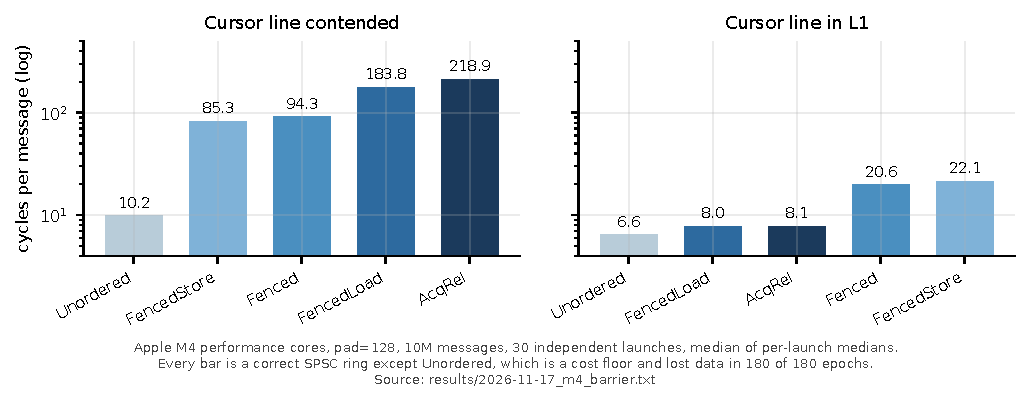
\includegraphics[width=\columnwidth]{fig-barrier.pdf}
\caption{Five correct rings and the cost floor, at both caching states, in
nanoseconds per message from the earlier run that first showed the reversal.
Contended the order is unordered 10.185, fencedstore 85.269, fenced 94.336,
fencedload 183.800, acqrel 218.880; resident it is unordered 6.646, fencedload
8.021, acqrel 8.053, fenced 20.567, fencedstore 22.120. The two arms that form
the comparison exchange places between the panels. Drawn from
\texttt{results/\allowbreak 2026-11-17\_\allowbreak m4\_\allowbreak barrier.txt}; the cycle-level replication of the
same comparison is in Section~\ref{sec:cycles}.}
\label{fig:barrier}
\end{figure}

\begin{table}[t]
\centering
\caption{Where the contended cost sits, in cycles per message, on each thread
of the ring. Waiting is cycles in which an older load or store is waiting for
data after an L1D miss. The arm that is cheaper overall is cheaper mostly by
waiting less, on both threads. From
\texttt{results/\allowbreak 2026-11-21\_\allowbreak m4\_\allowbreak h78\_\allowbreak storeprobe.txt} and
\texttt{results/\allowbreak 2026-11-21\_\allowbreak m4\_\allowbreak h79\_\allowbreak prodside.txt}.}
\label{tab:wait}
\begin{tabular}{lrrrr}
\hline
 & \multicolumn{2}{c}{consumer measured} & \multicolumn{2}{c}{producer measured} \\
arm & total & waiting & total & waiting \\
\hline
acq-rel & 217.755 & 139.0505 & 220.048 & 101.8133 \\
fenced-load & 185.786 & 113.4273 & 167.930 & 71.3838 \\
fenced & 94.340 & 35.8644 & 99.159 & 24.3877 \\
fenced-store & 80.894 & 32.5100 & 87.364 & 22.0050 \\
unordered & 10.186 & 5.2458 & 9.087 & 3.0079 \\
\hline
\end{tabular}
\end{table}

\subsection{The cost is time spent waiting, and it replicates across threads}

Table~\ref{tab:wait} gives the decomposition on both threads. Decomposing each arm into cycles spent waiting on the load-store unit after an
L1D miss and cycles spent elsewhere locates the effect. Contended, on the
consuming thread, the acquire-release arm costs 217.755 cycles per message of
which 139.0505 are waiting, and the fenced-store arm costs 80.894 of which
32.5100 are waiting, a waiting ratio of 0.2338. Of the cycles the faster arm
saves, 106.5 of 136.9 are cycles not spent waiting. The remainder is visible in
the non-waiting component, 78.704 against 48.384.

Counting is per thread on this unit, and the arms differ in the instruction the
producer executes, so the same measurement was repeated with the producer on the
measuring thread. There the acquire-release arm costs 220.048 cycles with
101.8133 waiting and the fenced-store arm 87.364 with 22.0050. The ordering of
the five arms is identical in both modes at both caching states and the sign of
the pair holds in 30 of 30 launches in each. Swapping which side is measured
moves magnitudes and moves neither the ordering nor the direction. From
\texttt{results/\allowbreak 2026-11-21\_\allowbreak m4\_\allowbreak h78\_\allowbreak storeprobe.txt} and
\texttt{results/\allowbreak 2026-11-21\_\allowbreak m4\_\allowbreak h79\_\allowbreak prodside.txt}.

\subsection{How long the run lasted decides which construct a reader would
choose}

The results above are all measured at ten million messages per epoch. That
choice is not neutral, and the size of the effect it carries is the largest
single number in this paper.

Figures~\ref{fig:runlength} and~\ref{fig:ordering} show the sweep. Sweeping run length with everything else fixed, the cost of the
acquire-release ring with the cursor line contended is 21.930 nanoseconds per
message at 200,000 messages, 133.860 at one million, 216.195 at five million
and 221.990 at ten million. The same ring with the line resident moves the
other way, 13.180, 19.370, 8.185 and 8.170. The ratio between the two caching
states therefore moves from 1.66 to 6.91 to 26.41 to 27.17 across the sweep, a
spread of 16.33 times between its smallest and largest value.

The consequence is not a widened error bar. It changes the answer. Ranking
three orderings at 200,000 messages gives acquire-release at 21.930, fenced at
86.280 and sequentially consistent at 178.795, so acquire-release is the
cheapest by a factor of four. Ranking the same three at ten million gives
221.990, 99.185 and 221.250, so acquire-release is the dearest and fenced is
the cheapest by more than a factor of two. A reader who benchmarked at 200,000
messages and a reader who benchmarked at ten million would recommend opposite
constructs, from the same binary on the same machine.

This hazard is not new and we do not claim it. Mytkowicz et
al.~\cite{mytkowicz2009wrong} established that an innocuous choice in an
experimental setup can reverse a conclusion, and found that none of 133 papers
they surveyed from ASPLOS, PACT, PLDI and CGO accounted for it. Run length is
such a choice, and on this part it is worth a factor of 16.33. Emurian et
al.~\cite{emurian2014pitfalls} identify the mechanism, which is that the core
clock responds to how long a core has been busy rather than to how much work it
was given, and bound the resulting distortion at about 8 percent on a
server-class part with up to 5.8 percent error on a nominal two times speedup.
On a fanless M4 the same mechanism produces 16.33 times, two orders of
magnitude larger, and it reverses conclusions rather than inflating margins. A
fanless part has no mechanism for sustaining a clock under load other than
lowering it.

The power state of that sweep was not recorded, because the harness began
capturing it two days afterwards, and on a fanless machine the power state
bounds the sustained clock. We therefore report the sweep as establishing that
the hazard is large on this class of machine, and not as a calibrated figure
for it. Every run after that date records its power state in its own header and
a gate checks every claim about it against the file. From
\texttt{results/\allowbreak 2026-11-16\_\allowbreak m4\_\allowbreak runlength.txt}.

\begin{figure}[t]
\centering
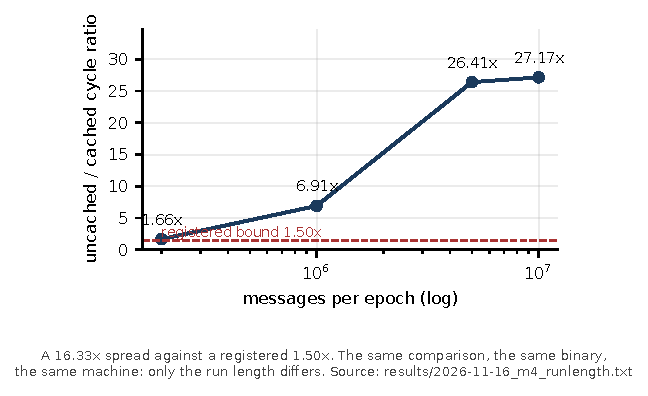
\includegraphics[width=\columnwidth]{fig-runlength.pdf}
\caption{Cost per message against run length, at both caching states. The
contended arm rises from 21.930 to 221.990 nanoseconds per message while the
resident arm falls from 13.180 to 8.170, so the ratio between them moves from
1.66 to 27.17. Drawn from
\texttt{results/\allowbreak 2026-11-16\_\allowbreak m4\_\allowbreak runlength.txt}.}
\label{fig:runlength}
\end{figure}

\begin{figure}[t]
\centering
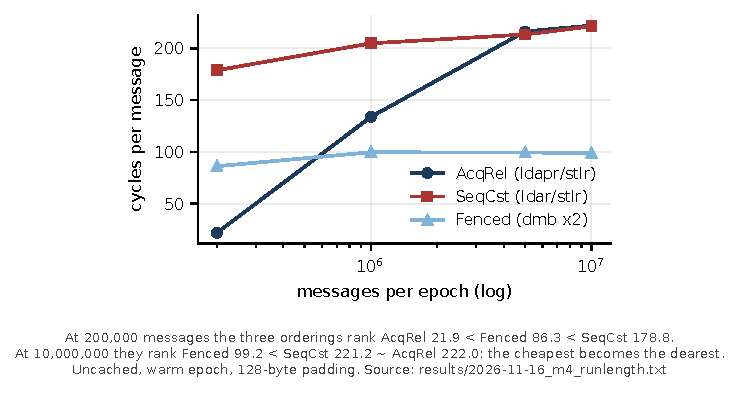
\includegraphics[width=\columnwidth]{fig-ordering.pdf}
\caption{The ranking of three orderings inverts with run length. At 200,000
messages the costs are 21.930, 86.280 and 178.795 nanoseconds per message for
acquire-release, fenced and sequentially consistent; at ten million they are
221.990, 99.185 and 221.250. A benchmark that stops early recommends the
opposite construct to one that does not. Drawn from
\texttt{results/\allowbreak 2026-11-16\_\allowbreak m4\_\allowbreak runlength.txt}.}
\label{fig:ordering}
\end{figure}

\subsection{What the counters rule out, and what they cannot reach}

The obvious explanation for a barrier arm that is faster is that it performs
less coherence work. Three attempts to test that on this part produced two
unmeasurable quantities and one that cannot distinguish cause from consequence,
and we report all three rather than the one that happened to yield a number.

Retired store misses are zero on every arm, on both threads, across 1800
records. The event counts stores that missed in L1D, and a miss requires the
line to be absent, while the ring stores into slots cycled through a small
buffer and into a cursor the thread writes continuously. A diagnostic whose
expected behaviour was fixed before the counter was read confirms the event
counts correctly in a workload built to miss, so the zero is a correct
measurement of a quantity this workload does not produce. Retired memory order
violations are likewise zero everywhere, and a validation pass with an aliasing
loop built to trigger them could not move the counter either, so that figure
supports no conclusion in either direction.

Writebacks of dirty lines from L1D do count, and per message the faster arm
performs roughly half as many, 0.9911 against 1.9808 on the producer and 0.4703
against 0.9933 on the consumer. That comparison cannot carry the mechanism.
Writebacks per message correlate with cycles per message at $r = 0.9966$ across
the producer cells and $r = 0.9879$ across the consumer cells, which is what
spinning on a remote cursor produces: a slower arm polls more times and moves
the line more often. A per-message rate of a quantity driven by duration,
compared between a fast arm and a slow one, measures the duration difference a
second time.

Controlling for duration removes the difference. Comparing the arms at matched
ring capacity, the writeback rate per cycle departs from unity by at most
1.2168, and at three of the five capacities by less than 1.14. An arm-specific
coherence component of that size cannot explain a cost difference of 2.5. We
therefore report that the mechanism is not identified by these measurements,
which is a weaker claim than the data initially appeared to support and the
only one it sustains. Ousterhout's rule is to measure one level
deeper~\cite{ousterhout2018deeper}, and doing so twice here first found a puzzle
and then found that the puzzle belonged to the instrument. Of the
acquire-release arm's contended cost, 7.77 percent of cycles are cycles in which
the scheduler issued at least one uop and 0.16 percent are cycles in which
nothing issued because of the backend, which leaves 92.07 percent in neither
state. One level deeper again, those cycles are frontend stalls. One level
deeper than that, they are an artifact of how the consumer waits: the frontend
share of the acquire-release arm's cycles is 0.9661 when the wait loop contains
an \texttt{isb} and 0.0542 when it does not, a factor of nearly eighteen, and
\texttt{isb} is context-synchronizing and forces an instruction refetch. The
stall profile of this ring under that wait strategy is mostly a measurement of
the wait strategy. With the \texttt{isb} removed both arms are backend bound and
the cost difference is accounted for by backend stall cycles, which is where a
memory-ordering effect should live, and Section~\ref{sec:wait} reports what does
and does not survive the change. From
\texttt{results/\allowbreak 2026-11-22\_\allowbreak m4\_\allowbreak h80\_\allowbreak viol\_\allowbreak prodside.txt},
\texttt{results/\allowbreak 2026-11-22\_\allowbreak m4\_\allowbreak h81\_\allowbreak viol\_\allowbreak consumer.txt} and
\texttt{results/\allowbreak 2026-11-22\_\allowbreak m4\_\allowbreak h84\_\allowbreak capfine.txt}.

\subsection{Which part of the ordering pair carries the cost}

The comparison so far has two arms, and two arms cannot say whether the cost
sits in the acquire or in the release. The arms differ on both sides at once:
one is an acquire load paired with a store-release, the other is the same
acquire load paired with a barrier and a plain store.

A third arm settles it, and it required no new code. Rust's sequentially
consistent ordering lowers on this part to \texttt{ldar}, the RCsc acquire,
which orders against earlier loads in a way \texttt{ldapr} does not. It is
strictly stronger than the acquire-release arm's load and it carries no
explicit barrier, so it sits between the two arms in ordering strength. The
implementation existed from the start and no arm list had ever dispatched it.

Contended, the three arms cost 204.493, 201.900 and 89.338 cycles per message
for acquire-release, sequential consistency and the fenced store. The ratio of
the middle arm to the first is 0.9873, against a bound of 0.90 registered in
advance as the point at which the two would be treated as one group, and the
fenced arm sits at 0.4369 in the same cells. Strengthening the acquire from
RCpc to RCsc costs 1.3\%. Moving the ordering to the store side changes the
cost by a factor of 2.29.

The launch-by-launch test agrees by failing. The sequentially consistent arm
is cheaper in 16 of 30 launches, p=0.8555 by the exact two-sided sign test,
against a registered 27 of 30. A difference of 1.3\% has no stable sign, which
is what it means for two arms to be one group, and had the point estimate
separated them this would have contradicted it.

So the ordering strength of the acquire is not what this paper is measuring.
Section~\ref{sec:cycles} reached the same place by decomposing the pair and
swapping one side at a time; this reaches it by adding a third ordering policy
that shares none of those arms. Both say the cost is on the store side.

\subsection{The comparison does not depend on how the consumer waits}
\label{sec:wait}

Every figure above is measured with one wait strategy, an \texttt{isb}-based
spin, and a parameter held constant across every run of a study is invisible
inside it. Varying it last is the reason this subsection exists.

Holding the arms fixed and varying only the wait strategy, the cost ratio of
the barrier arm to the release-store arm is 0.4161 under a plain spin, 0.3849
under the \texttt{isb} spin, 0.3945 under a yielding wait and 0.4532 under
\texttt{wfe}. The spin against \texttt{isb} comparison is 1.0809, inside a
registered band of 1.25, and the four values span less than a fifth of their
own size. The central result is a property of the ordering constructs and not
of the idling strategy, which no earlier run had established.

The stall decomposition does not survive the same test, and we report it as
conditional rather than quietly keeping it. The frontend share of the
acquire-release arm's cycles is 0.9661 under the \texttt{isb} wait and 0.0542
under a plain spin: a context-synchronizing instruction in the wait loop forces
an instruction refetch every iteration, and the arms differ in how many
iterations they spin. Under every wait strategy without one, both arms are
backend bound, and the ratio of backend stall cycles is 0.3511 under a plain
spin against a cost ratio of 0.4161, so the difference is accounted for by
backend stall and slightly over-accounted. That is a mechanism in the memory
system rather than the frontend, and it is what a reader would expect of a
memory-ordering experiment. We do not claim it, because it was found after the
thresholds that would have tested it were written, and fitting a threshold to
data already seen is the practice this protocol exists to prevent.

We do claim the correction it forces, and we ran it. The exclusion of pipeline
throttling rested on a ratio of issue-active fractions taken under the
\texttt{isb} wait. Re-measured across all four strategies with thresholds and
all three outcomes fixed beforehand, the acquire-release arm issues on 0.550940
of its cycles under a plain spin against 0.077303 under \texttt{isb}: the wait
loop suppressed the quantity the earlier comparison divided. The registered
outcome is inconclusive rather than confirmed or reversed, which is why that
threshold was written with three outcomes and not two.

\subsection{A boundary, and which property of the ring produces it}

The comparison is not a fixed property of the two instruction sequences. Swept
over ring capacity with the cursor line contended, its sign changes three times
across five capacities, as Table~\ref{tab:cap} shows. The acquire-release arm is
faster at capacity 2 in 20 of 20 launches and slower at capacity 1024 in 20 of
20, each at $p = 1.91\times10^{-6}$.

\begin{table}[t]
\centering
\caption{Cost per message in cycles, contended, by ring capacity. The sign of
the comparison changes three times and the acquire-release arm breaks
discontinuously between capacities 8 and 16. From
\texttt{results/\allowbreak 2026-11-22\_\allowbreak m4\_\allowbreak h84\_\allowbreak capfine.txt}.}
\label{tab:cap}
\begin{tabular}{rrrrr}
\hline
capacity & acq-rel & fenced-store & faster & advantage \\
\hline
2 & 153.838 & 165.898 & acq-rel & 1.0784 \\
4 & 91.997 & 86.072 & fenced-store & 1.0688 \\
8 & 63.972 & 76.105 & acq-rel & 1.1897 \\
16 & 173.725 & 71.194 & fenced-store & 2.4402 \\
1024 & 219.433 & 85.340 & fenced-store & 2.5713 \\
\hline
\end{tabular}
\end{table}

The break matters more than the sign change. The acquire-release arm falls from
153.838 cycles at capacity 2 to 63.972 at capacity 8 and jumps to 173.725 at
16, a factor of 2.716, with refills per message rising from 0.5254 to 2.0824
and writebacks from 0.2564 to 0.9985. The fenced-store arm moves by 0.935
across the same step. Whatever happens between 8 and 16 happens to one arm.

Capacity is not separable here by design alone. The slot type is eight bytes
and the region is page aligned, so capacity sets the footprint at 16, 32, 64,
128 and 8192 bytes, first filling a 128-byte line at exactly the capacity where
the break occurs, and it also sets how far the producer may run ahead. A second
design separates them: padding the slot to 128 bytes raises the footprint
sixteenfold while holding the slot count and the run-ahead. The break does not
survive it. The same capacity step costs 1.0057 padded, reaching the registered
threshold of 2.0 in 0 of 20 launches, against 2.0902 unpadded in 18 of 20,
$p = 4.0\times10^{-4}$, and writebacks and refills saturate at 1.0 and 2.0 per
message as the footprint reaches one line, then stay flat across a further
factor of sixteen. The break is a cache-line crossing. We registered the
opposite prediction, and its refutation is what identified the cause.

\section{Discussion}

\textbf{What a practitioner can take from this.} The usual guidance is to use
the weakest ordering that is sufficient, on the understanding that weaker is
cheaper. On this part that is not a performance rule. A store-release is
cheaper than a full barrier plus a plain store when the cursor line is resident
in L1, by 2.7008 in cycles, and more expensive when the line is contended, by
2.5766, and which regime a queue is in depends on how the threads are scheduled
rather than on anything in the source. The comparison also depends
non-monotonically on ring capacity: the arm that is faster at capacity 2 is
slower at capacity 16. The reading is therefore narrow and we state it narrowly.
On a fanless M4, for a single-producer single-consumer ring with padded cursors,
the ordering construct is not a constant factor and cannot be chosen once for
all configurations by strength alone. It must be measured in the configuration
it will run in.

\textbf{What the apparatus taught us.} Eight registered thresholds in this
study were precise, checkable, fixed before the data existed, and not tests of
the claims they were written for. One was written over five arms when the claim
concerned a pair; one over an absolute quantity when the claim concerned a
composition; one against the thread that does not execute the instruction under
test; one was a measurability guard scoped more widely than the comparison it
guarded; one normalised a quantity by the very thing under comparison, so the
comparison appeared twice in the answer; one cross-checked two counters whose
definitions do not make them proportional, so neither outcome could have meant
anything, and its registered consequence is recorded as void; one placed its
test on the single cell we judged cleanest while the claim was scoped over
every cell, and the registered cell missed the bound by 0.0200 while three of
four cleared it; and one compared the magnitude of a spread across three arms
when the claim concerned whether an effect persists, so it could not see that
the rank order of the arms reverses between conditions, and reported a pass on
a margin of one part in 7600.

Locating this against the literature takes care, because that literature has
already drawn a distinction nearby. Nosek et
al.~\cite{nosek2018preregistration} set out pre-registration as the separation
of hypothesis generation from testing.
Ledgerwood~\cite{ledgerwood2018distinguish} replied that two things are
conflated under one name: pre-registering a directional prediction, which makes
a theory falsifiable, and pre-registering an analysis plan, which controls the
type I error rate. Nosek et al.~\cite{nosek2018reply} accepted the
complementarity and argued a prediction without a plan is inert.

Every threshold above satisfies both halves. Each was a directional prediction,
and each came with a plan specific enough to execute without further choices:
cells, statistic, comparison and bound were written down and pushed before the
data existed. The failure is in neither half. It is in the join, in whether the
plan is a test of the prediction it was written under, and that join is not
what the exchange is about. Ledgerwood separates two things that can be
pre-registered; she does not ask whether the second tests the first, because in
those designs it generally does. On a machine with heterogeneous cores,
per-thread counters whose definitions are only partly documented, and a clock
that depends on history, it generally does not. Pre-registration protects
against moving a threshold after seeing data, and all eight were honoured
exactly as written. It does not protect against aiming a threshold at the wrong
quantity. The practice we arrived at is mechanical and we recommend it: before
a threshold is committed, state in one sentence what observation would make the
claim false, and confirm the threshold tests that sentence rather than a
quantity that merely moves with it.

\section{Threats to Validity}

\textbf{Scope.} Every measurement is from one machine, one part, one operating
system build and one compiler version, recorded in each results file header. We
make no claim about other Apple silicon generations, actively cooled parts, or
other architectures beyond two cross-architecture control runs. A single-part
study can establish that an effect exists there and bound its size; it cannot
establish prevalence.

\textbf{One parameter was constant in every run.} The protocol varies the
ordering arm, caching state, measured thread, ring capacity and, last, the wait
strategy. Adding that last axis showed it had been carrying two results: the
stall decomposition is substantially a measurement of the
context-synchronizing instruction in the wait loop, and the exclusion of
pipeline throttling rests on an issue-rate comparison that the same instruction
suppresses. Neither was visible while the parameter was fixed, because its
effect was credited to whatever moved against it. Both were re-measured against
thresholds written before the data existed. The cost ratios survived, moving by
1.0809 between the two extreme wait strategies inside a registered band of
1.25; the stall attribution did not, and the throttling exclusion returned
inconclusive. We state the general form because we expect it is common: a
parameter held constant across every run of a study cannot be seen inside that
study.

\textbf{What the counters describe.} Counting is per thread on this unit, so
every counter figure here is about one side of the ring and the side is named
wherever one is quoted. A registered threshold in this study was written
against the consumer while the arms differ in the producer's store, and
returned zero on every arm of nine hundred records before that was noticed.

\textbf{The mechanism is not identified.} We report a reproducible effect with
a located cost, mostly waiting on the load-store unit after an L1D miss, and no
cause. Coherence traffic is not supported: at matched ring capacity the
writeback rate per cycle departs from unity by at most 1.2168, which cannot
account for a difference of 2.5. Retired store misses and retired memory order
violations are unmeasurable on this part, and we treat them as unmeasured
rather than as evidence of absence.

\textbf{The padded arm moves more bytes.} Separating footprint from slot count
required a 128-byte slot, which also raises the bytes copied per message. Both
comparisons that carry the conclusion hold the slot size fixed on each side, so
neither is confounded by it, but no claim is made about the absolute cost of
the padded arms.

\textbf{Correctness testing does not establish ordering correctness.} The
unordered arm exists as a cost floor and is incorrect. Measured on the
consuming thread it produced a wrong sum in every record; with the threads'
roles exchanged and nothing else changed, it produced a correct sum in most of
them. Its incorrectness is a race and the schedule decides how the race
resolves. Passing a correctness check under one thread arrangement is not
evidence that a memory-ordering implementation is correct.

\textbf{Whether the cost floor is a fair baseline.}
The ordering fraction compares an incorrect arm against a correct one, so a
reader is right to ask whether the gap measures ordering or measures work the
compiler removed once it was free to reorder. The instruction census answers
it. On the consuming path the unordered arm emits 18 instructions against 19
for acquire-release, and on the producing path 20 against 23. Every arm carries
the same loop shape: two conditional branches, two compares, one pair load and
two returns. The compiler did not restructure the loop when the ordering was
removed; it deleted the ordering and left everything else standing.

One to three instructions of difference accompany a factor of 21 in cycles.
That disproportion is the point. If the unordered arm were cheap because less
work is done, the instruction counts would show it and they do not. The
fraction therefore bounds what the ordering semantics cost on this part, not
what the optimiser recovered, and the bound is what we claim.


\textbf{Statistics and resolution.} The inferential statistic throughout is the
exact two-sided sign test over independent launches, assuming only that
launches are exchangeable. Ninety-four hypothesis rows are registered, a
substantial minority recording refutations, and we apply no family-wise
correction: the headline results are at $p = 1.86\times10^{-9}$ and
$p = 1.91\times10^{-6}$ and survive any reasonable correction for a family of
this size, while a marginal row should be read as one test among many. The
launch count is reported with every sign test so a reader can apply their own.
The virtual counter advertises a one nanosecond tick and advances in units of
roughly 41.667 nanoseconds, with 0.7558 of consecutive reads not advancing; no
claim rests on a latency difference near that grain, and the cycle counts
carrying the central results come from the performance monitoring unit.

\section{Conclusion}

A store-release and a full barrier followed by a plain store are not ordered by
cost on this part. Which is cheaper depends on whether the cursor line is
contended, on which half of the ring the construct is changed, and on the ring's
capacity, and the comparison changes sign along all three. The effect is large,
2.5766 in cycles contended and 2.7008 in the other direction when resident, and
it reproduces across thirty independent launches and across both threads of the
ring.

Most of the cost difference is time spent waiting on the load-store unit after
an L1D miss, and we could not identify what produces that waiting. The
coherence traffic explanation does not survive controlling for duration, and the
two counters that would have tested the alternatives do not measure anything in
this workload. We report an effect with a location and without a mechanism,
which is less than we set out to find and is what the measurements support.

The study's other contribution is methodological and was not planned. Eight
pre-registered thresholds were honoured exactly and tested the wrong quantity,
and the register that records them is published with the paper so that the
failure mode can be criticised rather than inferred. Pre-registration in
systems measurement prevents a threshold from moving. It does not prevent a
threshold from pointing somewhere else, and that needs a separate discipline.

\bibliographystyle{IEEEtran}
\bibliography{refs}

\end{document}
